\documentclass[../calc3.tex]{subfiles}
\graphicspath{{\subfix{../figures/}}}
\begin{document}
\chapter{Vector Calculus}
\section{Vector Fields}
We will focus on the mathematical description for flow.

Examples are air flow (wind), fluid flow, and electromagnetic fields.

\begin{definition}[Vector Field]
    Written as $\vec{F}(x,y)=P(x,y)\vec{i}+Q(x,y)\vec{j} \rightarrow$ at each point $(x,y)$, there is a vector that depends on $x$ and $y$.
\end{definition}

\begin{example}
    Sketch $\vec{F}=x\vec{i}$.

    Basically at a point $x=1$, then the vector is $\vec{i}$ in the positive direction, the same applies for all $x$.
\end{example}

\ex Sketch $\vec{F}=\langle y,x\rangle$.

Of course, vector fields can be drawn in $3$-space.

Other notations are $\vec{F} = $vector field or if we associate $x,y$ with a radius vector, $\vec{F}(\vec{r})$.

\begin{example}
    We will look at inverse square fields.

    Newton's Law of Gravitation is defined $\left|\vec{F}\right|=\frac{mMG}{r^2}$, essentially particles of mass $m$ and $M$ attract each other with a force $\left|\vec{F}\right|$.

    Force exerted by particle of mass $M$ to particle of mass $m$ in the direction of a unit vector.

    The direction of this is $-\frac{\vec{r}}{\| \vec{r\|}}$.

    So we have $\left|\vec{F}(\vec{r})\right|=-\frac{mMG}{r^2}\cdot \frac{\vec{r}}{\| \vec{r}\|}$ and this is called the gravitational field.

    As a vector this is written as $\vec{F}(\vec{r})=\frac{c}{|\vec{r}|^3}\vec{r}$.
\end{example}

Recall the gradient is $\nabla f(x,y)=f_x(x,y)\vec{i}+f_y(x,y)\vec{j}$.

$\nabla f(x,y)$ is really a vector field in $2$-space and is called the gradient vector field.

\begin{example}
    Sketch the gradient field os $\phi(x,y)=x^2+y^2$.

    $\vec{\nabla}\phi = \langle 2x,2y\rangle$.

    This can be used to draw the gradient field.

    At each point, the vector points in the direction of maximum increase.
\end{example} 

Gradient vectors are long where level curves are close to each other. This is because the length of the gradient vector is equal to the value of the directional derivative.

\begin{definition}
    A vector field $\vec{F}$ is conservative in a region if it is the gradient field for some function $f$ in that region.

    $\vec{F}$ is conservative if $\vec{F}=\vec{\nabla}f$.

    $f$ is called a potential function of $\vec{F}$.
\end{definition}

\begin{example}
    Consider $\vec{F}=\langle 2x,y\rangle$. Is $\vec{F}$ conservative?

    If we can write $\vec{F}=\langle 2x,y\rangle = \vec{\nabla}f$, then it is conservative.

    If $f(x)=x^2+\frac{1}{2}y^2$, then $f_x=2x$ and $f_y=y$

    Therefore, $\vec{F}$ is conservative.
\end{example}

\section{Line Integrals}
What we know:
\begin{itemize}
    \item $\int$ is integrated over an interval
    \item $\iint$ is integrated over an area in $2$-space
    \item $\iiint$ is integrated over an area in $3$-space
\end{itemize}

Now, we are integrating along a curve in order to find mass, fluid flow, force.

Let us have a curve $C: x=x(t), y=y(t), a\leq t\leq b$.

We can integrate then as $\sum_{i=1}^{n}\left(x_i^*, y_i^*\right)\Delta s_i$, where $\Delta s_i$ is the length of subarc.

\begin{definition}
    If $f$ is defined on a smooth curve $C: x=x(t), y=y(t)$, then the line integral of $f$ along $C$ is:
    \[ \int\limits_{C} f(x,y)ds = \lim_{n\to\infty}\sum_{i=1}^n f\left(x_i^*,y_i^*\right)\Delta s_i \]
\end{definition}

Recall, arc length is $\int_a^b \sqrt{\left(\frac{dx}{dt}\right)^2+\left(\frac{dy}{dt}\right)^2}dt$.

So, $\int\limits_{C} f(x,y)ds = \int_a^b f(x(t),y(t)) \sqrt{\left(\frac{dx}{dt}\right)^2+\left(\frac{dy}{dt}\right)^2}dt$

Remember, $\frac{ds}{dt}=\sqrt{\left(\frac{dx}{dt}\right)^2+\left(\frac{dy}{dt}\right)^2}$, so $ds=\sqrt{\left(\frac{dx}{dt}\right)^2+\left(\frac{dy}{dt}\right)^2}dt$

\pagebreak
\begin{example}
    Evaluate $\int\limits_{C} (2+x^2y)ds$, where $C$ is the upper half of the unit circle.

    We need a parameterization of this curve. So $C: x=\cos t, y=\sin t$.

    The integral is $\int\limits_{C} (2+x^2y)ds = \int_0^{\pi} (2+\cos^2 t+\sin t)\sqrt{(-\sin t)^2+(\cos t)^2}dt$.

    This is equal to $\int_0^{\pi} 2+\cos^2 t\sin t dt = 2\pi + 2/3$.
\end{example}

\begin{example}
    Evaluate $\int\limits_{C} xds$ where $C$ is the portions of $y=x$ and $y=x^2$ from $(0,0)$ to $(1,1)$.

    Our first curve is $y=x$ and second curve is $y=x^2$.

    Let $c_1: y=x$, so the parameterization is $x=t, y=t, 0\leq t\leq 1$.

    So integrate $\int_0^1 t\cdot \sqrt{1^2+1^2}dt = \int_0^1 t\sqrt{2}dt = \frac{\sqrt{2}}{2}$.

    Let $c_2: y=x^2$. If we look at parameterization $x=t$ and $y=t^2$, we see that this will not work. So we have to parameterize as $x=1-t, y=(1-t)^2, 0\leq t\leq 1$.

    So we can integrate now $\int_0^1 (1-t)\sqrt{1+4(1-t)^2}dt$.

    Integrating this gives $\frac{1}{12}(5^{3/2}-1)$.

    Therefore, $\int\limits_{C} xdS = \frac{\sqrt{2}}{2}+\frac{1}{12}(5^{3/2}-1)$.
\end{example}

Right now, we have arc length parameterizations, so orientation does not matter. (For example, for $c_2$ above, we could have used parameterization $x=t, y=t^2$.)

What does this actually mean? It depends on the interpretation of the function $f$.
\begin{enumerate}
    \item If $f(x,y,z)$ represents density $\int\limits_{C} f(x,y,z)ds$ is the mass of a thin wire shaped like $C$.
    \item If $f(x,y)$ is a curve, then the area underneath the curve is $A=\int\limits_{C} f(x,y)ds$.
\end{enumerate}

So far we have calculated line integrals with respect to arc length: $\int\limits_{C} f(x,y)ds$.

We can also calculate line integrals with respect to $x$ and $y$:
\[ \int\limits_{C} f(x,y)dx = \int_a^b f(x(t),y(t))\cdot x'(t)dt\]
\[ \int\limits_{C} f(x,y)dy = \int_a^b f(x(t),y(t))\cdot y'(t)dt\]

Sometimes these occur together: $\int\limits_{C} P(x,y)dx+Q(x,y)dy$

\pagebreak
\begin{example}
    Evaluate $\int\limits_{C} y^2 dx + xdy$ along (a) $C_1$ and (b) $C_2$ where $C$ is as shown.
    \begin{center}
        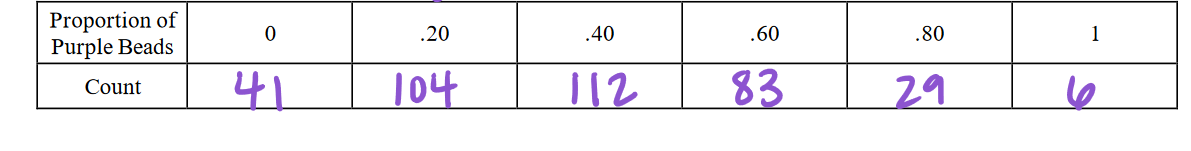
\includegraphics[width=0.3\textwidth]{5.1.1.PNG}
    \end{center}

    The curve $c_1$ is a line from $(-5,-3)$ to $(0,2)$.

    So $\vec{r}(t)=(1-t)\vec{r}_0+t\vec{r}_1, 0\leq t\leq 1$, $\vec{r}_0=\langle -5,-3\rangle, \vec{r}_1=\langle 0,2\rangle$.

    $\vec{r}(t)=\langle -5+5t,5t-3\rangle 0\leq t\leq 1$.

    So, $x=5t-5, y=5t-3$ and $dx=5dt$ and $dy=5$ with $0\leq t\leq 1$.

    So we can integrate $\int\limits_{C}y^2 dx + xdy$.

    This is $\int_0^1 [(5t-3)^2\cdot 5dt + (5t-5)\cdot 5 dt]=-\frac{5}{6}$.

    For $c_2$, let $y=t$ and $x=4-t^2$ for bounds $-3\leq t\leq 2$.

    What this gives us is $dy=1dt$ and $dx=-2tdt$.

    The integral for this is $\int_{-3}^2 [(t)^2(-2tdt)+(4-t^2)\cdot 1dt]$, which is equal to $\frac{245}{6}$.
\end{example}

This tells us that path matters. Line integrals in $3$-space are almost the same as $2$-space.

\begin{example}
    Evaluate $\int\limits_{C}y\sin zds$ where $C:x=\cos t, y=\sin t, z=t$ for $0\leq t\leq 2\pi$.

    $\int\limits_{C} y\sin zds = \int_0^{2\pi}\sin t\cdot \sin t\sqrt{(-\sin t)^2+(\cos t)^2+1^2}dt$.

    This is $\int_0^{2\pi}\sin^2 t\sqrt{2}dt$.

    This can be rewritten as $\sqrt{2}\int_0^{2\pi}\frac{1}{2}-\frac{1}{2}\cos 2t dt$.

    This is equal to $\sqrt{2}\pi$.
\end{example}

\begin{example}
    Evaluate $\int\limits_{C}ydx+zdy+xdz$ where $C$ consists of the line segment from $(2,0,0)$ to $(3,4,5)$, then the vertical line segment from $(3,4,5)$ to $(3,4,0)$.

    For the first curve we have $c_1: \vec{r}=(1-t)\langle 2,0,0\rangle + t\langle 3,4,5\rangle$ and $\vec{r}_1(t)=\langle 2+t,4t,5t\rangle 0\leq t\leq 1$.

    This gives $\int_0^1 4t\cdot 1 dt + 5t\cdot 4dt + (2+t)\cdot 5 dt = 24.5$.

    $c_2: \vec{r}=(1-t)\langle 3,4,5\rangle + t\langle 3,4,0\rangle$ and get $\vec{r}_2(t)=\langle 3,4,5-5t\rangle$.

    The integral is $\int_0^1 4(0dt)+(5-5t)(0dt)+3(-5dt) = -15$.

    The final answer is $24.5+-15 = 9.5$.
\end{example}

Recall: $W=\vec{F}\cdot \vec{d}$.

Now, suppose $\vec{F}=P\vec{i}+Q\vec{j}+R\vec{k}$ is a continuous force field (gravitational force field or electric force field).

We may want to calculate the work done in moving the particle among a smooth curve $C$.

\begin{definition}
    Let $\vec{F}$ be a continuous vector field defined on a smooth curve $C$ given by $\vec{r}(t)$.

    Then the line integral of $\vec{F}$ along $C$ is: $\int\limits_{C}\vec{F}\cdot d\vec{r}=\int_a^b \vec{F}(\vec{r}(t))\cdot \vec{r'}(t)dt = \int\limits_{C}\vec{F}\cdot \vec{T}ds$.

    This calculates work.
\end{definition}

\begin{example}
    Find the work done by $\vec{F}(x,y,z)=\left\langle -\frac{1}{2}x, -\frac{1}{2}y, \frac{1}{4}\right\rangle$ on a particle moving along the helix $\vec{r}(t)=\langle \cos t,\sin t, t\rangle, 0\leq t\leq 3\pi$.

    We have $\vec{r'}(t)=\langle -\sin t,\cos t, 1\rangle$ and $\vec{F}(\vec{r}(t))=\langle -\frac{1}{2}\cos t,-\frac{1}{2}\sin t,\frac{1}{4}\rangle$.

    So $W=\int\limits_C \vec{F}\cdot d\vec{r}=\int_0^{3\pi}\langle -\frac{1}{2}\cos t,-\frac{1}{2}\sin t,\frac{1}{4}\rangle\cdot \langle -\sin t,\cos t,1\rangle dt$.

    To simplify this, we have $\int_0^{3\pi}(\frac{1}{2}\cos t\sin t-\frac{1}{2}\sin t\cos t+\frac{1}{4})dt$.

    This is equal to $W=\frac{3}{4}\pi$.
\end{example}

Remark: $\int\limits_{C}\vec{F}\cdot d\vec{r}=-\int\limits_{-C}\vec{F}\cdot d\vec{r}$. If we reverse the path, work will be the opposite value.

\begin{example}
    Evaluate $\int\limits_{C}\vec{F}\cdot d\vec{r}$ where $\vec{F}=xy\vec{i}+yz\vec{j}+zx\vec{k}$ and $C:x=t, y=t^2,z-t^3,0\leq t\leq 1$.

    $\vec{r}=\langle t,t^2,t^3\rangle$, $\vec{r'}=\langle 1,2t,3t^2\rangle$, so $\vec{F}(\vec{r}(t))=\langle t^3,t^5,t^4\rangle$.

    So we end up getting $\int\limits_{C}\vec{F}\cdot d\vec{r}=\int_0^1 t^3+5t^6dt =\frac{27}{28}$.
\end{example}

Consider $\vec{F}=P\vec{i}+Q\vec{j}+R\vec{k}, \vec{r}(t)=\langle x(t),y(t),z(t)\rangle$.

Then $\int\limits_{C}\vec{F}\cdot d\vec{r}=\int_a^b \langle P,Q,R\rangle\cdot \langle x'(t),y'(t),z'(t)\rangle dt = \int_a^b (P\cdot x'(t)+Qy'(t)+R\cdot z'(t))dt$.

So $\int\limits_{C}\vec{F}\cdot d\vec{r}=\int\limits_{C}+Pdx+Qdy+Rdz$.

\begin{example}
    Calculate $\int\limits_{C}\vec{F}\cdot d\vec{r}$ where $\vec{F}=\langle \cos x,\sin x\rangle$ and $C: \vec{r}(t)=t\vec{i}+t^2\vec{j}, -1\leq t\leq 2$.
    
    $\vec{F}=\langle \cos t, \sin t\rangle$

    $\int\limits_{C}\vec{F}\cdot d\vec{r}=\int_{-1}^2 \langle \cos t, \sin t\rangle \cdot \langle 1,2t\rangle dt = \int_{-1}^2 \cos t + 2t\sin t dt$.

    When we integrate all of this we get $\sin t-2t\cos t+2\sin t$ from these bounds and the answer is $3\sin 2+3\sin 1-4\cos 2-2\cos 1$.
\end{example}


\section{The Fundamental Theorem for Line Integrals}
Recall the Fundamental Theorem of Calculus: $\int_a^b F'(x)dx = F(b)-F(a)$

Now, we have the Fundamental Theorem of Line Integrals.
\begin{theorem}[Fundamental Theorem of Line Integrals]
    Let $C$ be a smooth curve given by $\vec{r}(t)$, $a\leq t\leq b$. Let $f$ be a differentiable function whose gradient $\nabla f$ is continuous on $C$. Then $\int\limits_{C} \nabla f \cdot d\vec{r}=f(\vec{r}(b))-f(\vec{r}(a))$, where $f$ is a potential function.
\end{theorem}

\begin{example}
    Confirm that $f(x,y)=x^2y-\frac{1}{2}y^2$ is a potential function for $\vec{F}(x,y)=2xy\vec{i}+(x^2-y)\vec{j}$. Then evaluate $\int\limits_{C}\vec{F} \cdot d\vec{r}$ for $C$ where $C$ is a curve from $(-1,4)$ to $(1,2)$.

    The potential function is: $\vec{\nabla}f=\vec{F}$ and $\langle 2xy,x^2-y\rangle = \langle 2xy,x^2-y\rangle$.

    Then we can just see can integrate $\int\limits_{C}\vec{\nabla}f\cdot d\vec{r}$ and get $f(1,2)-f(-1,4)=4$.

    This value represents the work done in moving a particle from $(-1,4)$ to $(1,2)$. Previously we would have to use $\vec{r}(t)$ for a curve and parameterize and integrate.
\end{example}

Recall that $\int\limits_{C_1}\vec{F}\cdot d\vec{r}\neq \int\limits_{C_2}\vec{F}\cdot d\vec{r}$ (value of line integral depends on the path)

But: $\int\limits_{C_1}\nabla f\cdot d\vec{r}=\int\limits_{C_2}\nabla f\cdot d\vec{r}$ as long as $C_1$ and $C_2$ have the same endpoints (from the theorem above).

This is true for line integrals of a conservative vector field ($\vec{F}=\vec{\nabla}f$). In general, $\int\limits_{C}\vec{F}\cdot d\vec{r}$ is independent of path if $\int\limits_{C_1}\vec{F}\cdot d\vec{r}=\int\limits_{C_2}\vec{F}\cdot d\vec{r}$ for any $2$ paths $C_1$, $C_2$, that have the same initial points and endpoints.

Line Integrals along Closed Paths: The following are equivalent
\begin{enumerate}
    \item $\vec{F}(x,y)=\langle f(x,y), g(x,y)\rangle$ is conservative. 
    \item $\int\limits_{C}\vec{F}\cdot d\vec{r}=0$ (same initial/endpoint)
    \item $\int\limits_{C}\vec{F}\cdot d\vec{r}$ is independent of path from any point $P$ to any point $Q$.
\end{enumerate}

Any single one of these statements implies the other two statements for closed paths.

Simple Path: a path that goes from one point to another point.

Not Simple: A path that may curve back on itself.

Simply-Connected region: closed, non-intersecting 

Multiply-Conected region: region that has holes in the domain

So the theorem only applies when $\vec{F}$ is conservative. Then $\int\limits_{C}\vec{F}\cdot d\vec{r}=f(\vec{r}(b))-f(\vec{r}(a))$ where $\nabla f = \vec{F}$.

Conservative Field Test:

Let $\vec{F}(x,y)=P(x,y)\vec{i}+Q(x,y)\vec{j}$ be a vector field on an open, simply-connected region $D$. If $\frac{\partial P}{\partial y}=\frac{\partial Q}{\partial x}$ throughout $D$, then $\vec{F}$ is conservative.

\pagebreak
\begin{example}
    Show that $\vec{F}(x,y)=\langle 2xy^3,1+3x^2y^2\rangle$ is conservative. Then find the potential function.

    Previously, we would have found the potential function.

    We have $\frac{\partial P}{\partial y}=6xy^2$ and $\frac{\partial Q}{\partial x}=6xy^2$, so it is conservative.

    So integrating $\int\frac{\partial F}{\partial x}dx = \int 2xy^3 dx$ and get $f=x^2y^3+k(y)$.

    Now we can use $\frac{\partial f}{\partial y}=3x^2y^2+k'(y)$.

    So we cna see that this has to be equal to $3x^2y^2+k'(y)=1+3x^2y^2$.

    So we have $\int k'(y)=\int 1 dy$, so $k(y)=y+C$.

    Therefore, $f(x,y)=x^2y^3+y+C$.
\end{example}

\begin{example}
    Find the work done by the vector field $\vec{F}(x,y)=(y^3+1)\vec{i}+(3xy^2+1)\vec{j}$ in moving a particle from $(0,0)$ to $(2,0)$.

    Work is $\int\limits_{C}\vec{F}\cdot d\vec{r}$.

    Before, we would have parameterized.

    Now we can ask if $\vec{F}$ is conservative.

    $\frac{\partial P}{\partial y}=3y^2 = \frac{\partial Q}{\partial x}=3y^2$.

    Because the vector fields are conservative, then $\int\limits_{C}\vec{F}\cdot d\vec{r}=f(2,0)-f(0,0)$, where $\vec{\nabla f}=\vec{F}$.

    Start $\int \frac{\partial f}{\partial y}dy = \int 3xy^2+1 dy$ and we get $f=xy^3+y+k(x)$.

    Now $\frac{\partial f}{\partial x}=y^3+k'(x)=y^3+1$.

    So $\int k'(x)=\int 1 dx$ and $k(x)=x+C$.

    Therefore $f(x,y)=xy^3+y+x+C$.

    Work is $f(2,0)-f(0,0)=2-0=2$.
\end{example}

If $\vec{F}$ is conservative, then $\vec{F}$ is independent of path. If you cannot remember how to find $f$, choose any path from $(0,0)$ to $(2,0)$.

For example, we could have done $\vec{r}(t)=\langle 2t,0\rangle, 0\leq t\leq 1$, so work is $\int_0^1 \langle 1,1\rangle \cdot \langle 2,0\rangle dt = \int_0^1 2 dt = 2$.

Options for $\int\limits_{C} \vec{F}\cdot d\vec{r}$ (work)
\begin{enumerate}
    \item Parameterize Curve
    
    If $\vec{F}$ is conservative/independent of path 
    \item Find $f$ (potential function)
    \item Use any path from $P$ to $Q$
\end{enumerate}

\pagebreak
\begin{example}
    $\vec{F}=\langle y^2,2xy+e^{3z}, 3ye^{3z}\rangle$. Find $f$ such that $\nabla f = \vec{F}$.

    Let $f_x,f_y,f_z$ be the terms in $\vec{F}$ in order.

    So $\int f_x dx = \int y^2 dx$, or $f=xy^2+k(y,z)$.

    Now $f_y=2xy+k_y(y,z)=2xy+e^{3z}$.

    Integrating gives $\int ky(y,z)dy = \int e^{3z}dy$ so $k(y,z)=ye^{3z}+k(z)$.

    So right now we have $f=xy^2+ye^{3z}+k(z)$.

    So $f_z=3ye^{3z}+k'(z)=3ye^{3t}$ so $k'(z)=0$.

    Therefore $f(x,y,z)=xy^2+ye^{3z}+C$

    We can check by finding $f_x, f_y$, and $f_z$ from this.
\end{example}

\section{Green's Theorem}
George Green (1793-1841) was a self-taught british mathematician and physicist.

\begin{theorem}[Green's Theorem]
    Let $R$ be a simply connected plane region whose boundary is a simple, closed, piecewise smooth curve oriented counterclockwise.

    If $f(x,y)$ and $g(x,y)$ are continuous and have continuous first partials on some open set containing $R$, then 
    \[ \int\limits_{C}f(x,y)dx+g(x,y)dy = \iint\limits_{R}\left(\frac{\partial g}{\partial x}-\frac{\partial f}{\partial y}\right)dA \]
\end{theorem}
\begin{proof}
    We need to show $\int\limits_{C}f(x,y)dx = \iint\limits_{R}-\frac{\partial f}{\partial y}dA$

    Let $c_1$ and $c_2$ be boundary curves. Then $\int\limits_{C}f(X,y)dx=\int\limits_{c_1}f(x,y)dx+\int\limits_{c_2}f(x,y)dx$.

    This is equivalent to $\int\limits_{C}f(X,y)dx=\int\limits_{c_1}f(x,y)dx-\int\limits_{-c_2}f(x,y)dx$.

    When we parameterize this, we get $c_1: x=t, y=g_1(t)$ and $c_2: x=t, y=g_2(t)$.

    So the integral $\int\limits_{C}f(x,y)dx = \int_a^b f(t,g_1(t))dt - \int_a^b f(t,g_2(t))dt$.

    Then we have $-\int_a^b [f(t,g_2(t))dt-f(t,g_1(t))]dt$. This is equal to $-\int_a^b f(t,y)$ between the values $y=g_1(t)$ and $y=g_2(t)$ wrt $t$.

    We can write this now as a double integral $-\int_a^b \int_{g_1(t)}^{g_2(t)}\frac{\partial f}{\partial y}dy dx = -\iint\limits_{R}\frac{\partial f}{\partial y}dA$.
\end{proof}

\pagebreak
\begin{example}
    $\int\limits_{C}y^3 dx + (x^3+3xy^2)dy$ where $C$ is below. Also find $\int\limits_{C}\vec{F}\cdot d\vec{r}$ where $\vec{F}=\langle y^3,x^3+3xy^2\rangle$.

    $C$ goes from $(0,0)$ to $(1,1)$ and goes from the line $y=x$ then the line $y=x^3$.

    This is closed and counterclockwise, so we can use Green's Theorem.

    This integral becomes $\iint\limits_{R}\left(\frac{\partial g}{\partial x}-\frac{\partial f}{\partial y}\right)dA$.

    So we have $\iint\limits_{R}(3x^2+3y^2)-3y^2 dA = \int_0^1 \int_{x^3}^x 3x^2 dy dx = \frac{1}{4}$.

    For the other part, we need to do the line integral of $\int\limits_{C}\vec{F}\cdot d\vec{r}$.

    $\int\limits_{C}\vec{F}\cdot d\vec{r}=\frac{1}{4}$, it is basically the same as above.
\end{example}

If we have a closed path, then $\oint\limits_{C}f(x,y)dx+g(x,y)dy = \iint\limits_{R}\frac{\partial g}{\partial x}-\frac{\partial f}{\partial y}dA$.

Sometimes we get the orientation, such as $\ointclockwise\limits_{C}$ or $\ointctrclockwise\limits_{C}$.

If $\vec{F}$ is conservative, then $\oint\limits_{C}\vec{F}\cdot d\vec{r}=0$.

Another Application of Green's Theorem:

Area = $\iint\limits_{R}dA = \oint\limits_{C}xdy = \oint\limits_{C}-y dx = \frac{1}{2}\oint\limits_{C}-y dx + x dy$.

\begin{example}
    Use a line integral to find the area of $\frac{x^2}{a^2}+\frac{y^2}{b^2}=1$.

    This is an ellipse.

    If we parameterize this, we get $x=a\cos t$ and $y=b\sin t$ for $0\leq t\leq 2\pi$.

    We have $A=\oint x dy = \int_0^{2\pi}a\cos t\cdot b\cos t dt$.

    This is equal to $ab\int_0^{2\pi}\cos^2 t dt = ab\int_0^{2\pi}\left(\frac{1}{2}+\frac{1}{2}\cos 2t\right)dt$.

    This is equal to $A=\pi ab$.
\end{example}

For multiply-connected regions:
\begin{center}
    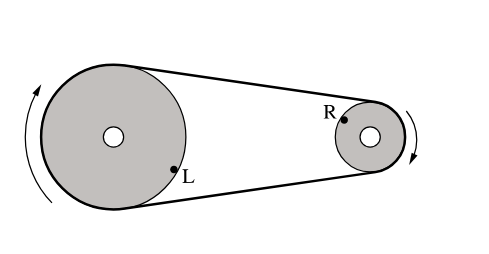
\includegraphics[width=0.3\textwidth]{5.2.PNG}
\end{center}

We want to calculate the line integral for this.

For the outside curve, we are finding $\oint\limits_{c_1}f(x,y)dx+g(x,y)dy$.

We have to go in and exit, so the inner region contributes nothing.

For the second curve, it is oriented clockwise so we have to reverse the orientation.

So we add $\oint\limits_{c_2}f(x,y)dx+g(x,y)dy$.

Using Green's Theorem, this becomes $\iint\limits_{R}\frac{\partial g}{\partial x}-\frac{\partial f}{\partial y}dA + \iint \frac{\partial f}{\partial y}-\frac{\partial g}{\partial x}dA$.

Now we will see is the curve has negative orientation and if we can use Green's Theorem.
\begin{example}
    Evaluate $\int\limits_{C}x^4 dx + xydx$ where $C$ is the triangle curve consisting of line segments from $(0,0)$ to $(0,1)$, to $(1,0)$, and then back to $(0,0)$.

    We need the curve to have the reverse orientation to use Green's Theorem.

    So we can just do $-\iint\limits_{-c}(y-0)dA = -\iint\limits_{R}ydA$.
\end{example}

\section{Curl and Divergence}
Let $\vec{F}=P\vec{i}+Q\vec{j}+R\vec{k}$. Then curl $\vec{F} = \vec{\nabla}\times \vec{F}$.

Curl relates to the rotational properties of a fluid at a point.

\begin{example}
    Find curl $\vec{F}$ for $\vec{F}=\langle xz,xyz,-y^2\rangle$.

    The cross product $\vec{\nabla}\times \vec{F}=\begin{vmatrix}
        \vec{i}& \vec{j}& \vec{k}\\
        \frac{\partial}{\partial x} & \frac{\partial}{\partial y}&\frac{\partial}{\partial z}\\
        xz & xyz & -y^2
    \end{vmatrix}$.

    This is equal to $\langle \frac{\partial}{\partial y}-\frac{\partial}{\partial z}(xyz),-[\frac{\partial}{\partial x}(-y^2)-\frac{\partial}{\partial z}(xz)], \frac{\partial}{\partial x}(xyz)-\frac{\partial}{\partial y}(xz)\rangle$.

    This is equal to curl $\vec{F}=\langle -y(2+x),x,yz\rangle$.
\end{example}

\begin{theorem}
    curl$(\nabla f)=\vec{0}$ (Note $f$ must have continuous 2nd order partials)
\end{theorem}
\begin{proof}
    curl$(\vec{\nabla}f)=\vec{\nabla}\times \vec{\nabla}f = \begin{vmatrix}
        \vec{i}&\vec{j}&\vec{k}\\
        \frac{\partial}{\partial x}& \frac{\partial}{\partial y}&\frac{\partial}{\partial z}\\
        \frac{\partial f}{\partial x} & \frac{\partial f}{\partial y} & \frac{\partial f}{\partial z}
    \end{vmatrix}$

    This is equal to $\langle \frac{\partial^2 f}{\partial y}{\partial z}-\frac{\partial^2 f}{\partial z\partial y}-\left(\frac{\partial^2 f}{\partial x \partial z}-\frac{\partial^2 f}{\partial z\partial x}\right), \frac{\partial^2 f}{\partial x \partial y}-\frac{\partial^2 f}{\partial y\partial x}\rangle$.

    Everything subtracts from each other, so $0\vec{i}+0\vec{j}+0\vec{k}$ is the result, or $\vec{0}$.
\end{proof}

We care about this because if $\vec{F}$ is a conservative vector field, then $\vec{\nabla f}=\vec{F}$.

So the theorem also says if $\vec{F}$ is conservative, then curl $\vec{F}=\vec{0}$.

\begin{theorem}
    If $\vec{F}$ is a vector field defined on all of $\mathbb{R}^3$ whose component functions have continuous partial derivatives and curl $\vec{F}=\vec{0}$, then $\vec{F}$ is a conservative vector field.
\end{theorem}

\begin{example}
    Show that $\vec{F}(x,y,z)=y^2z^3\vec{i}+2xyz^3\vec{j}+3xy^2z^2\vec{k}$ is conservative and find the potential function.

    Before, we would use $\vec{F}(x,y)=P\vec{i}+Q\vec{j}$ and find the partials.

    Now we can show in $3$-space that curl $\vec{F}=\vec{0}$.

    Remember that curl $\vec{F}=\vec{\nabla}\times \vec{F}$.

    This is equal to $\begin{vmatrix}
        \vec{i}&\vec{j}&\vec{k}\\
        \frac{\partial}{\partial x} & \frac{\partial}{\partial y} & \frac{\partial}{\partial z}\\
        y^2 z^3 & 2xyz^3 & 3xy^2z^2
    \end{vmatrix}$

    This gives $\langle 6xyz^2-6xyz^2, -(3y^2z^2-3y^2z^2), 2yz^3-2yz^3\rangle = \vec{0}$. $\vec{F}$ is a conservative vector field.

    Start with $\int f_x dx = \int y^2z^3 dx$, so $f=xy^2z^3+k(y,z)$.

    Now we have $f_y=2xyz^3+k'(y,z)=2xyz^3$, so then $\int k'(y,z)=\int 0$ so $k(y,z)=k(z)$.

    Now we have $f=xy^2z^3+k(z)$.

    $f_z=3xy^2z^2+k'(z)$ and from this we can see that $k'(z)=$ a constant.

    So our potential function is $f(x,y,z)=xy^2z^3+k$.
\end{example}

Divergence: div $\vec{F}=\vec{\nabla}\cdot \vec{F}$.

Divergence relates to the way in which fluid flows away or towards a point.

\begin{example}
    Find div $\vec{F}$ for $\vec{F}=\langle xz,xyz,-y^2\rangle$.

    So div $\vec{F}=\vec{\nabla}\cdot \vec{F}=\langle \frac{\partial}{\partial x}, \frac{\partial}{\partial y},\frac{\partial}{\partial z}\rangle \cdot \langle xz,xy^2,-y^2\rangle$.

    This gives us div $\vec{F}=z+xz+0$, so div $\vec{F}=z+xz$. This is called a scalar field.
\end{example}

Laplacian: $\nabla^2$

$\nabla^2 = \vec{\nabla}\cdot \vec{\nabla}=\frac{\partial^2}{\partial x^2}+\frac{\partial^2}{\partial y^2}+\frac{\partial^2}{\partial z^2}$.

If applied to $f(x,y,z)\rightarrow \nabla^2 f = \frac{\partial^2 f}{\partial x^2}+\frac{\partial^2 f}{\partial y^2}+\frac{\partial^2 f}{\partial z^2}$.

So, $\nabla^2 f =$ div$(\vec{\nabla}f)$.

Vector Forms of Green's Theorem:

Consider $\vec{F}=P\vec{i}+Q\vec{j}$. Suppose all conditions for Green's Teorem are satisfied. Then 
\[ \oint\limits_{C}\vec{F}\cdot d\vec{r}=\int\limits_{C}Pdx+Qdy=\iint\limits_{D}(Q_x-P_y)dA \]

curl $\vec{F} = \begin{vmatrix}
    \vec{i} & \vec{j} & \vec{k}\\
    \frac{\partial}{\partial x} & \frac{\partial}{\partial y} & \frac{\partial}{\partial t}\\
    P(x,y) & Q(x,y) & 0
\end{vmatrix} = \left(\frac{\partial Q}{\partial x}-\frac{\partial P}{\partial y}\right)\vec{k}$.

So we can rewrite Green's theorem as: 
\[ \oint\limits_{C}\vec{F}\cdot d\vec{r}=\iint\limits_{D}(\text{curl}\vec{F})\cdot \vec{k}dA \]
This is equal to $\iint\limits_{D}\left(\frac{\partial Q}{\partial x}-\frac{\partial P}{\partial y}\right)\vec{k}\cdot \vec{k}dA$ or $\iint\limits_{D}\frac{\partial Q}{\partial x}-\frac{\partial P}{\partial y}dA$.

\section{Surface Integrals}
Recall: $\int, \iint, \iiint, \int\limits_{C}ds$, or ($\int\limits_{C}d\vec{r}$ or $\oint\limits_{C}$ - Green's theorem)

The idea now is integrating over a smooth parametric surface.

Take $\vec{r}(u,v)=x(u,v)\vec{i}+y(u,v)\vec{j}+z(u,v)\vec{k}$.

Then form Riemann sum: $\sum_{i=1}^m\sum_{j=1}^n f\left(P_{ij}^*\right)\Delta S_{ij}$.

If we take the limit $\lim_{m,n\to \infty}\sum_{i=1}^m\sum_{j=1}^n f\left(P_{ij}^*\right)\Delta S_{ij}$ this becomes equal to $\iint\limits_{S}f(x,y,z)dS$.

The above expression represents the surface integral of $f$ over $S$.

To evaluate:
\begin{enumerate}
    \item If parameterize: $\iint\limits_{S}f(x,y,z)dS = \iint\limits_{D}f(\vec{r}(u,v))|\vec{r}_u\times \vec{r}_v|dA$. (Note $|\vec{r}_u\times \vec{r}_v|$ denotes the surface area of a surface $S$)
    \item If rectangular: $\iint\limits_{S}f(x,y,z)dS = \iint\limits_{D}f(x,y,g(x,y))\sqrt{\left(\frac{\partial z}{\partial x}\right)^2 + \left(\frac{\partial z}{\partial y}\right)^2 + 1}dA$
\end{enumerate}

Interpretation:
\begin{enumerate}
    \item Mass 
    \item $\iint\limits_{S}dS$ is surface area 
    \item Mass/center of mass: $m=\iint\limits_{S}\rho(x,y,z)dS$ and $\overline{x}=\frac{1}{m}\iint\limits_{S}x\cdot \rho(x,y,z)dS$
\end{enumerate}

\begin{example}
    Evaluate $\iint\limits_{S}x^2 dS$ over the sphere $S: x^2+y^2+z^2=1$.

    Let $x=\sin\phi cos\theta$, $y=\sin\phi\sin\theta$ and $z=cos\phi$.

    So $\vec{r}(\phi,\theta)$.

    So cross product $\vec{r}_\phi \times \vec{r}_\theta = \begin{vmatrix}
        \vec{i}&\vec{j}&\vec{k}\\
        \cos\phi\cos\theta & \cos\phi\sin\theta & -\sin\phi \\
        -\sin\phi\sin\theta & \sin\phi\cos\theta & 0
    \end{vmatrix} = $
    
    $\langle \sin^2\phi\cos\theta,\sin^2\phi\sin\theta, \sin\phi\cos\phi\cos^2\theta + \sin\phi\cos\phi\sin^2\theta\rangle$.

    So we get $\langle \sin^2\phi\cos\theta, \sin^2\phi\sin\theta, \sin\phi\cos\phi\rangle$.

    So the magnitude of this is $\sqrt{\sin^4\phi\cos^2\theta+\sin^4\phi\sin^2\theta+\sin^2\phi\cos^2\phi}=\sqrt{\sin^4\phi+\sin^2\phi\cos^2\phi}=\sqrt{\sin^2\phi}=\sin\phi$.

    Now we have $\iint\limits_{S}x^2 dS = \int_0^{2\pi}\int_0^{\pi}(\sin\phi\cos\theta)^2\cdot \sin\phi d\phi d\theta$.

    This is equal to $\int_0^{2\pi}\cos^2\theta d\theta \cdot \int_0^{\pi}\sin^3\phi d\phi$.

    The first integral gives $\int_0^{2\pi}\left[\frac{1}{2}+\frac{1}{2}\cos 2\theta\right]d\theta = \pi$.

    The second integral becomes $\int_0^{\pi}\sin\phi(1-\cos^2\phi)d\phi = \int_0^{\pi}(\sin\phi-\sin\phi\cos^2\phi)d\phi = \frac{4}{3}$.

    These are being multiplied, so $\pi\cdot \frac{4}{3}=\frac{4}{3}\pi$.
\end{example}
\pagebreak
\begin{example}
    Evaluate $\iint\limits_{S}(y^2+2ys)dS$ where $S$: first octant of $2x+y+2z=6$.

    We will use the $\iint\limits_{D}f(x,y,g(x,y))$ to solve this.

    We have $z=\frac{1}{2}(6-2x-y)$ and $z_x=-1, z_y=-\frac{1}{2}$. Then we have $\sqrt{1^2+\frac{1}{2}^2+1}=\frac{3}{2}$.

    The surface integral becomes $\iint\limits_{D} [y^2+2y(\frac{1}{2}(6-2x-y))]\cdot \frac{3}{2}dA$.

    We end up getting $\frac{3}{2}\int_0^3 \int_0^{6-2x} (y^2+6y-2xy-y^2)$.

    This evaluates to $\frac{243}{2}$.
\end{example}

Surface Integrals of Vector Fields:

Main Applications:
\begin{enumerate}
    \item Line integrals calculate work.
    \item Surface integrals calculate flux.
\end{enumerate}

Flow Fields - think about $\vec{F}(x,y,z)$ representing velocity of a fluid particle at the point $(x,y,z)$.

Oriented Surface:

``orientable'': surface has $2$ sides (outside and inside)

``non-orientable'': one side only 

$\vec{n}$ is a unit vector at each point. $-\vec{n}$ is a unit normal vector in opposite direction. Unit normals will never have an abrupt change in direction.

Orientation of a smooth parametric surface is defined by $\vec{n}$.

$\vec{n}=\frac{\vec{r}_u\times \vec{r}_v}{|\vec{r}_u\times \vec{r}_v|}$ gives a unit vector with a positive orientation.

\begin{example}
    Find the natural orientation for $\vec{r}(u,v)=\langle \cos u, v,-\sin u\rangle, 0\leq u\leq 2\pi, 0\leq v\leq 3$.

    The cross product is $\vec{r}_u\times \vec{r}_v = \begin{vmatrix}
        \vec{i} & \vec{j} & \vec{k}\\
        -\sin u & 0 & -\cos u\\
        0 & 1 & 0
    \end{vmatrix}=\langle \cos u, 0,-\sin u\rangle$.

    The magnitude $|\vec{r}_u\times \vec{r}_v| =1$ and $\vec{n}=\langle \cos u,0,-\sin u\rangle$.

    When $u=0, v=0$, then $\vec{n}=\langle 1,0,0\rangle$.

    Outward is positive orientation at this point, and negative is inward.
\end{example}

Flux conditions:
\begin{itemize}
    \item We will only deal with incompressible fluids (uniform density)
    \item We will assume that the velocity of a fluid at a fixed point does not vary with time (steady-state)
\end{itemize}

\pagebreak
\begin{definition}[Flux]
    The volume of a fluid that passes through a surface in one unit of time.

    This depends on 
    \begin{enumerate}
        \item speed of fluid (greater speed gives greater volume)
        \item how surface is positioned relative to flow. Maximum flux is when fluid is perpendicular to surface and no flux happens when nothing is passing through.
        \item Area of surace (larger area gives more flux)
    \end{enumerate}
\end{definition}

How do we calculate flux?

Flux = $\phi = \iint\limits_{S}\vec{F}\cdot d\vec{S} = \iint\limits_{S}\vec{F}\cdot \vec{n}dS = \iint\limits_{D}\vec{F}\cdot \frac{\vec{r}_u\times \vec{r}_v}{|\vec{r}_u\times \vec{r}_v|}|\vec{r}_u\times \vec{r}_v|dA$

Flux: $\phi = \iint\limits_{S}\cdot d\vec{S}=\iint\limits_{D}\vec{F}\cdot (\vec{r}_u\times \vec{r}_v)dA$

\begin{example}
    Find the flux of the vector field $\vec{F}(x,y,z)=z\vec{i}+y\vec{j}+x\vec{k}$ across the unit sphere $x^2+y^2+z^2=1$.

    Writing in terms of $\phi$ and $\theta$, we have $r(\phi,\theta)=\langle \sin\phi\cos\theta,\sin\phi\sin\theta,\cos\phi\rangle$.

    Crossing gives $\vec{r}_{\phi}\times \vec{r}_{\theta}=\begin{vmatrix}
        \vec{i}&\vec{j}&\vec{k}\\
        \cos\phi\cos\theta & \cos\phi\sin\theta & -\sin\phi \\
        -\sin\phi\sin\theta & \sin\phi\cos\theta & 0
    \end{vmatrix} = \langle \sin^2\phi\cos\theta,\sin^2\phi\sin\theta, \sin\phi\cos\phi\rangle$.

    So $\phi=\iint\limits_{S}\vec{F}\cdot d\vec{S}=\iint\limits_{D}\vec{F}\cdot (\vec{r}_u\times \vec{r}_v)dA$

    We have that $\vec{F}(\vec{r}(\phi,\theta))\cdot (\vec{r}_{\phi}\times \vec{r}_{\theta})=\cos\phi\sin^2\phi\cos\theta + \sin^3\phi\sin^2\theta + \sin^2\phi\cos\phi\cos\theta$.

    Flux is $\int_0^{2\pi}\int_0^{\pi}(\cos\phi\sin^2\phi\cos\theta + \sin^3\phi\sin^2\theta + \sin^2\phi\cos\phi\cos\theta)d\phi d\theta$.

    We can pull out some things and get $2\int_0^{2\pi}\sin^2\phi\cos\phi d\phi \cdot \int_0^{2\pi}\cos\theta + \int_0^{\pi}\sin^3\phi d\phi\cdot \int_0^{2\pi}\sin^2\theta d\theta$.

    Simplifying this gives $\int_0^{\pi}\sin^3\phi d\phi \cdot \int_0^{2\pi}\sin^3\theta d\theta = \frac{4\pi}{3}$.
\end{example}

Now for Non-Parametric Surfaces:

Suppose $z=g(x,y)$ is a surface oriented upward. Rewrite this function as $z-g(x,y)=0$.

For $\vec{n}$, use $\vec{n}=\frac{\langle -z_x-z_y,1\rangle}{|\sqrt{z_x^2+z_y^2+1} |}$. If we call $z-g(x,y)=0$ as $G(x,y,z)$, then $\vec{n}=\frac{\vec{\nabla}G}{|\vec{\nabla}G |}$.

So, if oriented upwards, $\iint\limits_{S}\vec{F}\cdot \langle -z_x,-z_y,1\rangle dA$. Downwards, we get $\iint\limits_{S}\vec{F}\cdot \langle z_x,z_y,-1\rangle dA$.

\pagebreak
\begin{example}
    Evaluate $\iint\limits_{S}\vec{F}\cdot d\vec{S}$ where $\vec{F}=\langle y,x,z\rangle$ and $S$ is the boundary of the solid region $E$ enclosed by $z=1-x^2-y^2$ and $z=0$. Assume outward orientation.

    When we draw this, we can call the upwards orientation $s_1$ and the downwards orientation $s_2$.

    For $s_1$: $\iint\limits_{s_1}\vec{F}\cdot d\vec{s}$.

    This is $\iint\limits_{D}\langle y,x,1-x^2-y^2\rangle\cdot \langle 2x,2y,1\rangle dA = \iint\limits_{D}(2xy+2xy+1-x^2-y^2)dA$.

    This is equal to $\iint\limits_{D}(1+4xy-x^2-y^2)dA$. Polar will make this integral easier.

    The integral becomes $\int_0^{2\pi}\int_0^1 (1+4r^2\cos\theta\sin\theta-r^2)\cdot dr d\theta = \frac{\pi}{2}$.

    For $s_2$, we have $z=0$.

    So we can rewrite $\iint\limits_{s_2}\vec{F}\cdot d\vec{s}=\iint\limits_{D}\langle y,x,0\rangle\cdot \langle 0,0,-1\rangle dA$.

    This is $\iint\limits_{D}0dA =0 $.

    So, the flux is $\frac{\pi}{2}$.
\end{example}

\section{Stokes' Theorem}
Recall: $\oint\limits_{C}\vec{F}\cdot d\vec{r}=\iint\limits_{R}\left(\frac{\partial Q}{\partial x}-\frac{\partial P}{\partial y}\right)dA$. 

Green's theorem applies for closed curves $C$ on the $xy$-plane.

We previously talked about writing Green's Theorem as $\oint\limits_{C}\vec{F}\cdot d\vec{r}=\iint\limits_{R}\text{curl}\vec{F}\cdot \vec{K}dA$.

We could do this because $\begin{vmatrix}
    \vec{i}&\vec{j}&\vec{k}\\
    \frac{\partial}{\partial x} & \frac{\partial}{\partial y}&\frac{\partial}{\partial z}\\
    P & Q & 0
\end{vmatrix} = \langle 0,0,\frac{\partial Q}{\partial x}-\frac{\partial P}{\partial y}\rangle \cdot \langle 0,0,1\rangle$.

So, Green's theorem can be tied to curl.

Recall the right-hand rule, the surface on the left is the positive orientation.

\begin{theorem}[Stokes' Theorem]
    Let $S$ be an oriented piecewise smooth surface bounded by a curve $C$ with positive orientation.

    \[ \int\limits_{C}\vec{F}\cdot d\vec{r}=\iint\limits_{S}\text{curl}\vec{F}\cdot d\vec{s}\]
\end{theorem}

\pagebreak
\begin{example}
    $\vec{F}(x,y,z)=\langle x^2,4xy^3,xy^2\rangle$. Find the work done by $\vec{F}$ on a partial traversing $z=y$ as shown.

    \begin{center}
        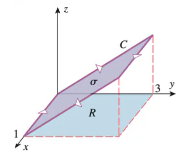
\includegraphics[width=0.3\textwidth]{5.3.PNG}
    \end{center}

    Previously, we could have used Green's theorem if the curve was on the $xy$-plane. 

    We could have also parameterized the $4$ lines and set up $4$ line integrals.

    Using Stokes' Theorem, we must ask if the surface is smooth (yes), do we have a curve with positive orientation (yes if $\vec{n}$ is down).
    
    So we have $W=\int\limits_{C}\vec{F}\cdot d\vec{r}=\iint\limits_{S}\text{curl}\vec{F}\cdot d\vec{s}$.

    Finding curl$\vec{F}=\langle 2xy,-y^2,4y^3\rangle$.

    To find $d\vec{s}$, we find $\langle z_x,z_y,-1\rangle = \langle 0,1,-1\rangle$.

    So the integral becomes $W=\iint\limits_{R}\langle 2xy,-y^2,4y^3\rangle\cdot \langle 0,1,-1\rangle dA = \int_0^1 \int_0^3 (-y^2-4y^3)dy dx = -90$.
\end{example}

\begin{example}
    Evaluate $\int\limits_{C}\vec{F}\cdot d\vec{r}$ where $\vec{F}(x,y,z)=-y^2\vec{i}+x\vec{j}+z^2\vec{k}$ and $C$ is the curve of intersection of $y+z=2$ and $x^2+y^2=1$. Orient $C$ to be counterclockwise when viewed from above.

    \begin{center}
        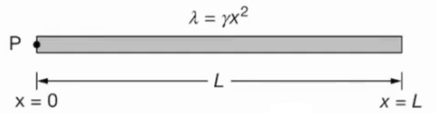
\includegraphics[width=0.3\textwidth]{5.4.PNG}
    \end{center}

    The surface is smooth, and the curve $c$ has positive orientation so Stokes' theorem can be used.

    The curl$\vec{F}$ is $\langle 0,0,1+2y\rangle$.

    $y+z=2$ gives $z=2-y$, and since $\vec{n}$ is up, we have $\langle -z_x,-z_y,1\rangle = \langle 0,1,1\rangle$.

    So the line integral is $\int\limits_{C}\vec{F}\cdot d\vec{r}=\iint\limits_{D}\langle 0,0,1+2y\rangle \cdot \langle 0,1,1\rangle dA$.

    This is $\iint\limits_{D}(1+2y)dA$. Since the region is a circle, polar is a good option.

    So we have $\int_0^{2\pi}\int_0^1 (1+2r\sin\theta)\cdot r dr d\theta = \pi$
\end{example}

$\oint\limits_{C}\vec{F}\cdot d\vec{r}=\iint\limits_{R}\left(\frac{\partial Q}{\partial x}-\frac{\partial P}{\partial y}\right)dA$ is a special case of Stokes' Theorem.

\begin{example}
    Verify Stokes' Theorem for $\vec{F}(x,y,z)=\langle 2z,3x,5y\rangle$ where $S: 4-x^2-y^2, z\geq 0$, upward orientation and $C: x^2+y^2=4$ on $xy$-plane (positively oriented).

    We start with $\vec{r}=\langle 2\cos t,2\sin t,0\rangle$.

    We use $\int\limits_{C}\vec{F}\cdot d\vec{r}=\int\vec{F}(\vec{r}(t))\cdot \vec{r'}(t)dt$.

    So the integral is $\int_0^{2\pi} 12\cos^2 t dt$ after the dot product and this is equal to $12\pi$.

    Using $\iint\limits_{S}\text{curl}\vec{F}\cdot d\vec{s}$ should give us similar answer.

    The curl$\vec{F}$ is $\langle 5,2,3\rangle$, and $S$ has upward orientation, so $\langle -z_x,-z_y,1\rangle = \langle 2x,2y,1\rangle$.

    So the integral is $\iint\limits_{R}\langle 5,2,3\rangle\cdot \langle 2x,2y,1\rangle = \iint\limits_{R}(10x+4y+3)dA$.

    The integral is $\int_0^{2\pi}\int_0^2 (10r\cos\theta+4r\sin\theta+3)r dr d\theta = 12\pi$.
\end{example}

\begin{example}
    $\iint\limits_{S}\text{curl}\vec{F}\cdot d\vec{S}$ for $\vec{F}=\langle xz,yz,xy\rangle$ where $S$ is the part of sphere $x^2+y^2+z^2=4$ that lies inside $x^2+y^2=$ above the $xy$-plane.

    We can use a line integral for this.

    We need to find $c$ first:

    $x^2+y^2+z^2=4$ and $x^2+y^2=1$, so $1+z^2=4$, so we can get $z=\sqrt{3}$ from this.

    So $C: x^2+y^2=1, z=\sqrt{3}$.

    We have $\vec{r}=\langle \cos t,\sin t,\sqrt{3}\rangle$, so $\vec{r'}(t)=\langle -\sin t,\cos t,0\rangle$.

    Therefore $\int\limits_{C}\vec{F}\cdot d\vec{r}=\int_0^{2\pi}\langle \sqrt{3}\cos t,\sqrt{3}\sin t,\cos t\sin t\rangle\cdot \langle -\sin t, \cos t,0\rangle dt$.

    This is equal to $\int_0^{2\pi}(-\sqrt{3}\cos t\sin t+\sqrt{3}\sin t\cos t)dt = 0$.
\end{example}

\section{The Divergence Theorem}
Recall that given $\vec{F}(x,y,z)=\langle f(x,y,z), g(x,y,z), h(x,y,z)\rangle$, that div$\vec{F}=\frac{\partial f}{\partial x}+\frac{\partial g}{\partial y}+\frac{\partial h}{\partial z}$ (fluid flow)

\begin{theorem}[Divergence Theorem]
    Let $E$ be a solid (closed) and let $S$ be the boundary surface of $E$, given with positive (outward) orientation. Then 
    \[ \phi = \iint\limits_{S}\vec{F}\cdot d\vec{S}=\iiint\limits_{E}\text{div}\vec{F}dV \]

    This is like using the potential function to calculate work when you have a conservative vector field.
\end{theorem}

\pagebreak
\begin{example}
    Find the flux of the vector field $\vec{F}(x,y,z)=z\vec{i}+y\vec{j}+x\vec{k}$ over the unit sphere $x^2+y^2+z^2=1$. We will assume outward orientation.

    It is closed and div$\vec{F}=0+1+0=1$.

    The flux is $\iint\limits_{S}\vec{F}\cdot d\vec{S}=\iiint\limits_{E}1\cdot dV$.

    $E$ is unit sphere $x^2+y^2+z^2\leq 1$ and $S$ is boundary $x^2+y^2+z^2=1$.

    The options are set up bounds (spherical coordinates) or to find the volume with a triple integral noting the volume of a sphere is $V=\frac{4}{3}\pi r^3$.

    The flux is $\frac{4}{3}\pi$.
\end{example}

\begin{example}
    Find the (outward) flux of the vector field $\vec{F}=\langle x,y^2,z\rangle$ across $S$: tetrahedron bounded by $2x+2y+z=6$ in the $1$st octant.

    Divergence theorem can be used because the solid is closed. div$\vec{F}=2+2y$.

    Flux is $\int_0^3 \int_0^{3-x} \int_0^{6-2x-2y} (2+2y)dz dy dx$.

    The answer of the integral is $31.5$.
\end{example}

\begin{example}
    Evaluate $\iint\limits_{S}\vec{F}\cdot d\vec{S}$ where $\vec{F}=\langle xy,y^2+e^{xz^2},\sin(xy)\rangle$ and $S$ is the surface of the region bounded by $z=1-x^2,z=0,y=0$, and $y+z=2$.
\begin{center}
        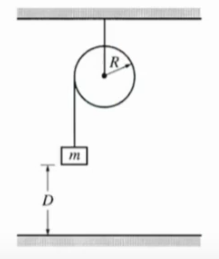
\includegraphics[width=0.3\textwidth]{5.5.PNG}
    \end{center}

    We get div$\vec{F}=3y$.

    The flux is $\phi = \iint\limits_{S}\vec{F}\cdot d\vec{S}=\int_{-1}^1 \int_0^{1-x^2} \int_0^{2-z} 3y dy dz dx$.

    The answer is $\frac{184}{35}$.
\end{example}

Sources and Sinks

A source is a point where fluid enters flow. (div$\vec{F}(p_0)>0$)

A sink is a point where fluid leaves flow. (div$\vec{F}(p_0)<0$)

\begin{example}
    Determine if $\vec{F}=(y+z)\vec{i}-xz^3\vec{j}+(x^2\sin y)\vec{k}$ is free of sources and sinks. If not, locate them.

    We have div$\vec{F}=0$, so there are no sources and no sinks.
\end{example}

\begin{example}
    Find all sources and sinks for $\vec{F}(x,y,z)=\langle xy,-xy,y^2\rangle$.

    The divergence of $\vec{F}$ is div$\vec{F}=y-x$.

    Sources will happen when $y-x>0$ and sinks will happen when $y-x<0$.

    So sources at all points where $x<y$ and there are sinks at all points where $x>y$.
\end{example}

\end{document}